\section{Debugging and testing}
\subsection{Instruction Memory test bench}

In the test bench, we iterated through all the memory addresses (including the out-of-bounds ones) and checked if the output was as expected:
\begin{code}[16]{}
initial begin
	$monitor("address=%d, instruction=%b\n", Address, Instruction);
	for (Address = 0; Address < 40; Address = Address + 1) begin
		#10;
	end
end
\end{code}
During the testing, we did not find any issues.
\subsection{Register File Test Bench}
This final part has been added mainly for debugging and testing our Register File.\newline

\begin{code}{Testing and Debugging}[47]
    generate
		genvar i;
		for (i = 0; i < r; i = i + 1) begin
		assign DebugData[i * l +: l] = Data[i[2:0]];
		end
	endgenerate
\end{code}

\subsection{Control Unit Test Bench}

In our implementation of the test bench, we went through all the possible opcodes and checked if the module output was correct.
\begin{code}[27]{Test Bench of Control Unit}
initial begin
    $monitor("LoadUpperImmediate=%d\nALUOpcode=%d\nUseImmediate=%d\nUpdateFlags=%d\n\n", LoadUpperImmediate, ALUOpcode, UseImmediate, UpdateFlags);
    
    $display("MUL:");
    Opcode = 3'b111;
    #10;
    ...
\end{code}
During the testing, we didn't find any issues.

\subsection{Addition Test Bench}
 In implementing the test bench, we went through all the possible edge cases, which are overflow, carry or overflow and carry at the same time.
 \begin{code}[20]{Addition Test Bench}
initial begin
	$monitor("  a=%b\n  b=%b\nsum=%b, o=%b, c=%b\n\n", a, b, sum, overflow, carry);
  ...
           
		x = 16'b1000000000110000;
		y = 16'b1000000011100000;
            #10;
  ...
		x = 16'b0111111111111111;
		y = 16'b0000000000000001;
		#10;
		x = 16'b1111111111111111;
		y = 16'b0000000000000001;
            #10;
	end
    ...
\end{code}
\subsection{Multiplication Test Bench}
In implementing the test bench, we went through all the possible edge cases, which is overflow. To make the overflow easier to detect we used in our test bench 3-bit integers.
 \begin{code}[23]{Multiplication Test Bench}
initial begin
...
		$monitor("X=%d,\nY=%d\nR1=%d, O=%b\n", X, Y, R1, Overflow);
  ...
		X = 16'd3;
		Y = 16'd4;
            #10;
    ...
\end{code}


\begin{figure*}[b]
	\centering
	\fbox{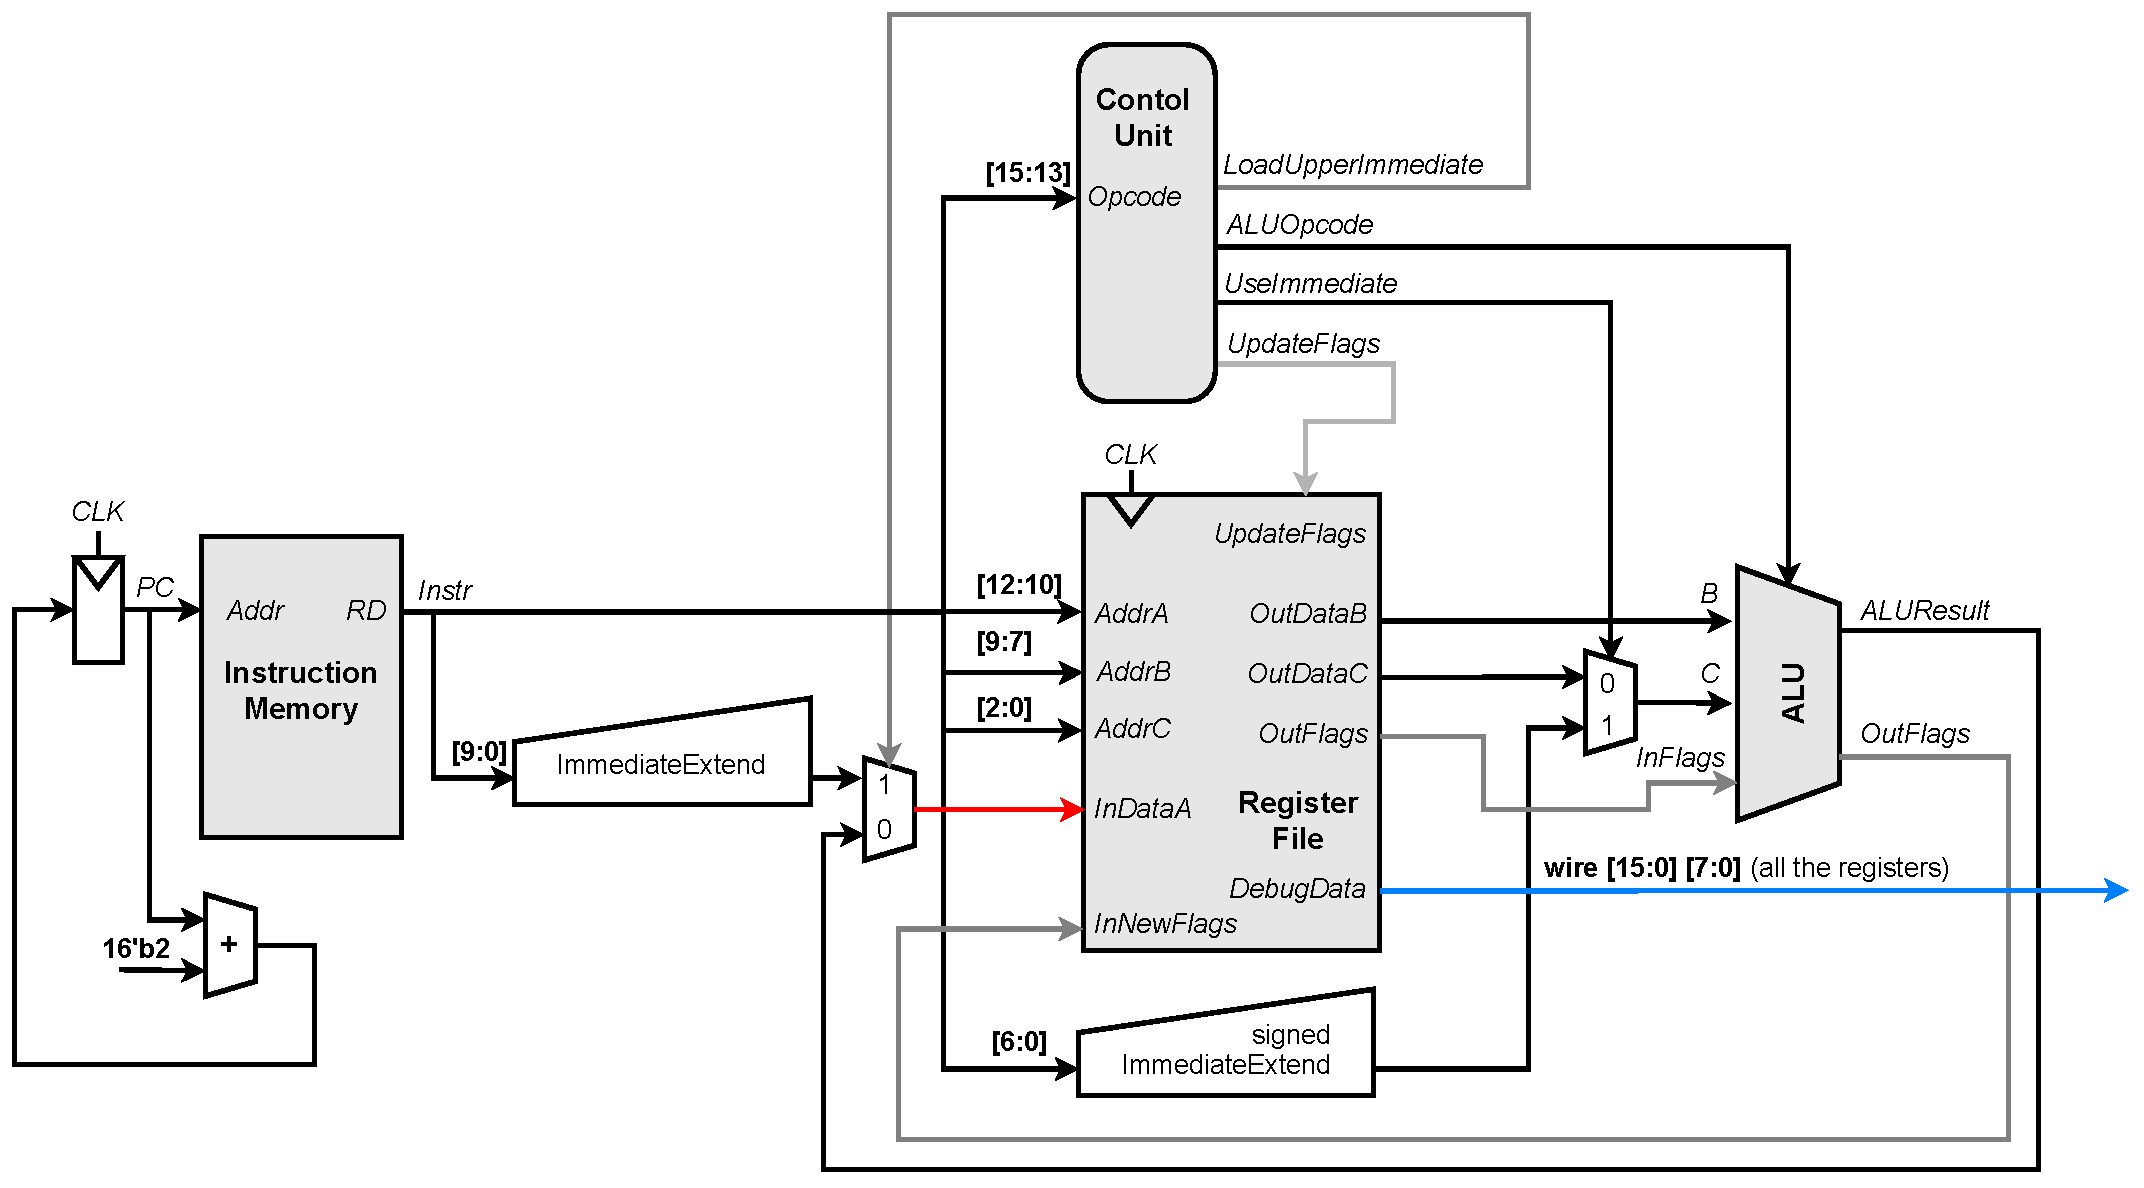
\includegraphics[width=.9\textwidth]{pics/diagrams/riscv/riscv.pdf}}
	\caption{Diagram of the RISC-V module.}
	\label{fig:riscv}
\end{figure*}

\subsection{Division Test Bench}
In implementing the test bench, we went through all the possible edge cases, which is divByzero and remainder. 
 \begin{code}[17]{Division Test Bench}
	initial begin
		$monitor("min=%d\ndiv=%d\nq=%d, r=%b, z=%b\n\n", min, div, quotient, HasRemainder, DivByZero);
		min = 16'd0;
		div = 16'd0;
		#10;
  ...
		min = 16'd7;
		div = 16'd0;
  	    #10;
		min = 16'd5;
		div = 16'd2;
            #10;
    ...
\end{code}
\subsection{ALU Test Bench}
In implementing the test bench, we went through all the possible edge cases of multiplication and division to make sure that all modules are connected and work correctly.